%\documentclass{article}
\documentclass[conference]{IEEEtran}
\usepackage{graphicx} % Required for inserting images
\usepackage{epstopdf}
\usepackage{float}
\usepackage{verbatim}
\usepackage{IEEEtrantools}
\usepackage[
    backend=biber,
    style=ieee,
  ]{biblatex}
\addbibresource{additional.bib}  % Additional papers (those not found in SLR)
\usepackage{svg}

\usepackage{xcolor}
\usepackage{longtable}

\begin{document}

%\begin{table}
%\begin{tabular}{|l|l|l|}
%\hline
%\textbf{Events}                                 & \textbf{Points} & \textbf{Obtained} \\ \hline
%Group formation                                 & 0.5               &   0.5               \\ \hline
%Topic selection, case study/ paper selection    & 0.5               &   0.5              \\ \hline
%Survey completion/ Experimentation and analysis & 02               &  1.5                \\ \hline
%Critical Assessment & 02               &           1.5       \\ \hline
%First draft                                     & 02               & -                 \\ \hline
%Second draft                                    & 01               & -                 \\ \hline
%\end{tabular}
%\end{table}
 
\title{Shifting Gears: A Systematic Literature Review of Process Model Transitioning in Software Engineering}

% APPARENTLY THIS IS THE WAY IT IS SUPPOSED TO BE DONE WITH MORE THAN 3 AUTHORS
\author{
\IEEEauthorblockN{Clayton Asada\IEEEauthorrefmark{1},
Aaron Trank\IEEEauthorrefmark{2},
Joseph Chorbajian\IEEEauthorrefmark{3},
Frederik Juul Stokbaek\IEEEauthorrefmark{4} 
Anthony Reyes\IEEEauthorrefmark{5} and
Christopher De Jong\IEEEauthorrefmark{6}}
\IEEEauthorblockA{\IEEEauthorrefmark{1}Computer Engineering and Computer Science\\
California State University Long Beach\\
clayton.asada01@student.csulb.edu}
\IEEEauthorblockA{\IEEEauthorrefmark{2}Computer Engineering and Computer Science\\
California State University Long Beach \\
aaron.trank01@student.csulb.edu}
\IEEEauthorblockA{\IEEEauthorrefmark{3}Computer Engineering and Computer Science\\
California State University Long Beach \\
joseph.chorbajian01@student.csulb.edu}
\IEEEauthorblockA{\IEEEauthorrefmark{4}Computer Engineering and Computer Science\\
California State University Long Beach \\
FrederikJuul.Stokbaek01@student.csulb.edu
}
\IEEEauthorblockA{\IEEEauthorrefmark{5}Computer Engineering and Computer Science\\
California State University Long Beach \\
anthony.reyes02@student.csulb.edu
}
\IEEEauthorblockA{\IEEEauthorrefmark{6}Computer Engineering and Computer Science\\
California State University Long Beach \\
christopher.dejong@student.csulb.edu
}
}


\date{February 2023}



\maketitle

%\begin{itemize}
%\color{blue}
%
%
%
%\color{brown}
%\item In fig. 1, text on blue background is not readable.
%\item You need to target conferences/journals, check their page limit, and revise your draft accordingly. Usually, the journal article is 15-25 pages long, and the conference paper can be 10-15. 
%\item Highlight the findings/ challenges/ issues from the downloaded papers.
%
%\color{red}
%\item Missing students' affiliations and email addresses.  
%\begin{itemize}
%    \item FIXED ...ALSO JUST ADD CORRECT EMAILS
%\end{itemize}
%\item The abstract should include the context, problem, method, result, and conclusion.
%\begin{itemize}
%    \item SORTA FIXED; WE NEED TO FOCUS OUR CONCLUSION. I THINK WE SHOULD SAY THERE IS A MISMATCH WITH REAL WORLD AND LITERATURE
%\end{itemize}
%\item The introduction section's last paragraph should be a paper walk-through. The introduction section should highlight the problem state and contribution. 
%\begin{itemize}
%    \item FIXED; ADDED ADDITIONAL PARAGRAPH TO COVER PROBLEM STATE AND CONTRIBUTION
% \end{itemize}
%\item Please make the reference consistent; it should be the last section.
%\begin{itemize}
%    \item IT IS THE LAST SECTION SO IDK WHAT TO DO ABOUT THIS
%\end{itemize}
%\item Table 2's caption should be on top of the table like you did with Table 1. 
%\begin{itemize}
%    \item FIXED
%\end{itemize}
%\item Some figures have borders like Fig. 2, and some are not like Fig. 3. Make them consistent. 
%\begin{itemize}
%    \item FIXED
%\end{itemize}
%\item Table 3 format is different from Tables 1 and 2. Make them consistent. 
%\begin{itemize}
%    \item FIXED
%\end{itemize}
%\item Labels on Fig. 2, 3, 4, 6, and 7 are inconsistent. In Fig. 6, the black text on a dark blue background is not readable. If the reader takes a printout (black/white), it will not be readable. 
%\begin{itemize}
%    \item FIXED
%\end{itemize}
%\item Figures 10 and 11, and 12 and 13 differ in format.
%\begin{itemize}
%    \item HE MIGHT NOT LIKE IT BUT I THINK SOME VARIATION IN THE CHARTS IS OK
% \end{itemize}
%\item Make the terminology consistent. If the figure caption is Fig. 1, then in the discussion, it should be referred to as Fig. 1 instead of Figure 1. 
%\begin{itemize}
%    \item FIXED
% \end{itemize}
%\item Paper should be cited before closing the sentence like "....success [10]."
%\begin{itemize}
%    \item FIXED
% \end{itemize}
%\item You have cited very few papers. I suggest citing more papers in the introduction section. You should also highlight how your work differs from other survey papers. For that you can create a section Related Work and then differentiate your contribution.
%\begin{itemize}
%    \item FIXED; added more references around the paper and included 90\% of selected papers as part of how we made the questionnaire
% \end{itemize}
%\item I think Findings should be a separate section. 
%\begin{itemize}
%    \item NOT SURE WHAT TO SAY ABOUT THIS.... IT IS
% \end{itemize}
%\item The empirical study is the main strength of your work. I think it will be a good idea if you highlight your audience (amazon, etc.).
%\item I suggest using the word practitioners instead of colleagues. 
%\begin{itemize}
%    \item FIXED
% \end{itemize}
%\item It will be okay if you remove the opening and closing dates of the survey.
  

%\end{itemize}

\begin{abstract}
Process models are essential in guiding teams through the software development process. Initial process models, such as the waterfall model, offered clear and defined stages that must be completed sequentially before the next. However, they fail at being flexible and adaptable to the needs of businesses and its consumers. Newer process models are designed with versatility in mind, reflecting the ever-changing requirements of the software development industry, in hopes to improve the speed and quality of products.
The transition between process models can be a complex and time-consuming process that requires careful coordination and training for many teams. Despite challenges, many teams recognize the benefits of newer process models that can help them respond to changing market demands.
In our research we conduct a systematic literature review to find the current state of process model transitioning. Key concepts and findings are extracted from SLR identified papers to create an empirical study survey, which was administer to practitioners remotely at Amazon and Experian. The responses were analyzed and compared with the current research literature to determine if research literature was properly covering real world problems and challenges. Our finding show a disconnect between the current literature and realities experienced by process model practitioners and suggest areas for further research.
% TODO: Maybe include most prominent results/analyses in abstract?

\emph{Keywords - } Waterfall, Agile, Transition, Process Model
\end{abstract}

\section{Introduction}
Software development is a highly dynamic field which, over time, has required more flexibility and adaptability to meet the growing demands of businesses and consumers\cite{9753613}. One of the most important aspects of software development is the process model. The process model defines a road map for teams to follow, outlining the steps that must be taken and their sequence. The road map helps teams ensure that they are following the best practices and meeting project goals.

Originally, software was developed using a linear and sequential approach, following steps of requirements gathering, defining, planning, executing, testing, and finally delivery\cite{8672701}. Each step must be fully completed before moving on to the next. This approach, known as the waterfall model, suffers from long return on investment periods and runs the risk of delivering a product which does not meet current needs. To overcome these shortcomings, newer process models have emerged that are incremental and iterative, where each step of the process is repeated in a cycle, continually and consistently delivering an improved product.

While the transition to a new process model can bring significant benefits, it is not always straightforward\cite{6702805}. Each process model has its own unique challenges, and transitioning to a new model requires careful consideration and planning. This may involve adapting existing processes and practices, training teams in new skills and techniques, and changing communication and collaboration methods.

Despite the potential challenges of transitioning from one process model to another, the benefits of using a process model which is appropriate for a given project are clear. Matching the correct process model to a given project helps teams deliver software more efficiently, with fewer defects, within budget, and on schedule. Due to the effects a process model can have on such important project metrics, software development organizations should regularly evaluate their process models and make adjustments as needed to ensure that they are using the most effective approach for their needs\cite{10049356}.

The subsequent research is an SLR aimed at identifying what the current state of literature does and does not cover in terms of transitioning between process models. Through the SLR conducted, a gap in the literature is found in the subject of transitioning from one process model to a different process model. An empirical survey of working professionals is conducted to compare real world experiences of practitioner to what is written in the literature. Again a disparity is shown between current research and current reality. Finally we conclude that more research is needed on process model transition and that further analysis should be conducted to identify important aspects of transitioning, as key highlighted factors in literature where not reflected as important in the empirical study responses.

\section{Motivation}
Our research team is driven to look into how software development teams can switch between various process models, stemming from our own difficult experiences with such transitions. We think that businesses and software development teams can tremendously benefit from knowing how to shift from one process paradigm to another and to another and so on. The lack of research studying transitions between different process models quickly, and the realization that certain process models may be better suited to various projects or stages of a project, are the driving forces fueling our interest in this area. The importance of companies adapting to new practices and procedures while switching between process models was highlighted in papers \cite{chen2010} and \cite{AFZAL2009957}.

While there has been considerable attention on research regarding process modeling and improvement, most of it has concentrated on the creation and use of specific process models. Research on the difficulties involved in switching between process models is not very extensive, outside of waterfall to agile transitions. Due to shifting business needs, developing technologies, and other external influences, many organizations today must quickly switch between process models. As a result, there is a considerable vacuum in the literature.

Our goal is to assist development teams in understanding the potential benefits of transitioning to process models that better align with their project and to make knowledgeable decisions about how to transition between them as project requirements change by examining the process of switching between different models. By investigating the transition between process models, which can aid in tearing down silos and encourage cross-functional teams to cooperate more closely, we also hope to enhance collaboration and communication within development teams. We are also interested in discovering the best techniques and methods for ensuring a seamless transition and overcoming the difficulties involved with moving to and from various process models.

The potential significance of this research excites our team, and we look forward to adding to the body of knowledge in this field. We seek to advance our understanding of software development processes and assist firms in remaining competitive in a market that is changing quickly through our investigation of process model transitions. In order to improve project outcomes, strengthen team collaboration and communication, and stay current with industry best practices, our research team is highly motivated to look into the process of switching between various process models in software development.


\section{Research methodology}
Two methodologies were used in this paper: a systematic literature review and an empirical study through a questionnaire. The systematic literature review will analyze existing approaches and problems on process model transitioning. The empirical study will collect further information from people who may have participated in a process model transition. The sections below describe what is done for both approaches.


\subsection{Systematic literature review}
Systematic literature review (SLR) is a research methodology involving a rigorous and comprehensive search of existing literature in a specific research area. The studies are chosen according to inclusion and exclusion criteria that align with research questions \cite{KHAN2017180, kitchenham}. This is done to reduce likelihood of systematic error. The findings of an SLR can produce relevant studies that can be further analyzed to answer research questions in that area. SLR is widely used in many fields, including healthcare and software engineering \cite{kitchenham}.

This paper follows the guidelines for a SLR proposed by Kitchenham et. al. \cite{kitchenham}. Notably, SLR is split into three phases: planning the review, conducting the review, and reporting the review \cite{kitchenham}. All authors took part in the three phases of the SLR. To guide the process, some points from CRD's \cite{university2001undertaking} checklist were used.

\subsubsection{Planning Phase}

\paragraph{Research questions}
Based on the aforementioned motivation for this paper, we crafted the following research questions.

\textbf{RQ1} \textit{What are the existing approaches to process model transitioning in software engineering?} In answering this question we hope to better understand \textbf{how} organizations transition to new process models.

\textbf{RQ2} \textit{What are the challenges of process model transitioning in software engineering?} In answering this question we hope to better understand \textbf{what} challenges organizations face when transitioning to a new process model.

\textbf{RQ3} \textit{What are the benefits of process model transitioning in software engineering?} In answering this question we hope to better understand \textbf{why} organizations choose to transition to new process models.

\paragraph{Sources Used}
The search was conducted between February 22 and March 31, 2023 on the IEEE Xplore, ACM Digital Library, and Springer Link research databases. IEEE Xplore, ACM Digital Library, and Springer Link are three popular research databases for conducting searches for SLR. The three databases both act as an indexer for their respective publishers' (IEEE, ACM, Springer) and for other publishers papers. Additional index engines, such as Google Scholar, have considerable overlap and were not used \cite{chen2010}.

\paragraph{Search String}
The research databases were searched with the following string: ("Abstract":waterfall OR "Abstract":agile OR "Abstract":iterative OR "Abstract":extreme OR "Abstract":lifecycle) AND ("Abstract":transition OR "Abstract":changing OR "Abstract":switch OR "Abstract":vs OR "Abstract":increase OR "Abstract":improvement) AND ("Abstract":waterfall OR "Abstract":agile OR "Abstract":iterative OR "Abstract":extreme OR "Abstract":lifecycle)

\paragraph{Criteria for Selection}
After running the search string in the databases, each paper goes through the selection process. The paper selection process uses the tollgate approach proposed by Afzal et al. \cite{AFZAL2009957}. Table \ref{tab:SLRSteps} illustrates the steps taken in the process. After the search is performed, any duplicates from the databases were removed, leaving only one unique instance of the paper. For the purpose of counting, the first database that showed the paper is counted as its origin. Next, the articles are selected based on the title. If the paper  does not seem irrelevant, then the paper's abstract will be examined. If no exclusion criteria is matched, then it will be processed for quality assessment.

For a paper to be selected, it must meet the following criteria:
\begin{itemize}
\item The papers must be in English and be available to access by the authors.
\item The papers must be published between 2013 and 2023.
\end{itemize}
Additionally, papers would have been excluded if they meet any of the following criteria:
\begin{itemize}
\item The paper is not about software engineering. Certain phrases, such as agile or waterfall, are used in other contexts. % TODO: Should we find a source for this?
\item The paper does not discuss about process model transitioning. As a consequence, papers discussing only one software process model were excluded.
\end{itemize}

\begin{table}[h!]
    \label{tab:SLRSteps}
    \caption{SLR - Search and selection process}
    \begin{tabular}{l p{4.4cm} r}
        \hline
         \textbf{Step} & \textbf{Description} & \textbf{\# papers IEEE/ACM} \\
         \hline
         1 & Perform search by contents of abstract & 3589\\
         2 & Remove duplicates and papers published after 2013 & 1157\\
         3 & Select articles based on titles & 315 \\
         4 & Select articles based on abstracts & 44 \\
         5 & Apply quality assessment criteria \\
         \hline
    \end{tabular}
\end{table}

\subsubsection{Conducting Phase}
\paragraph{Quality Assessment}
After obtaining a subset of relevant papers, each author was tasked with determining whether to select a given paper for further analysis or not, based on the contents of the research paper's abstract. The three options were:
\begin{itemize}
\item Yes. The paper is relevant to the research questions on process model transitioning.
\item Maybe. The paper may have been relevant to one or more of the research questions, but may not have had process model transitioning as the focus of the paper.
\item No. The paper is not relevant to the research or is unable to help with one of the research questions, despite the title and abstract alluding to its usefulness.
\end{itemize}
Each author was assigned an even split of papers and tasked to quality assess the papers by the abstract using these quality assessment questions in table \ref{tab:QAQ}.

\begin{table}[h!]
    \centering
    \label{tab:QAQ}
    \caption{Questions for quality assessment}
    \begin{tabular}{l p{7.3cm} r} 
        \hline 
        \textbf{ID}  &  \textbf{Question}\\ \hline
        QA1 & Does the paper include software process model/s \\[2mm]
        QA2 & Does the paper address the topic of process model transitioning \\[2mm]
        QA3 & Does the study highlight challenges in model transitioning \\[2mm]
        QA4 & Are the findings relevant to the research question?
        \\[2mm] \hline
    \end{tabular} \vspace{2mm}
\end{table}

\vspace{10mm}
\begin{figure}[h!] 
    \centering
    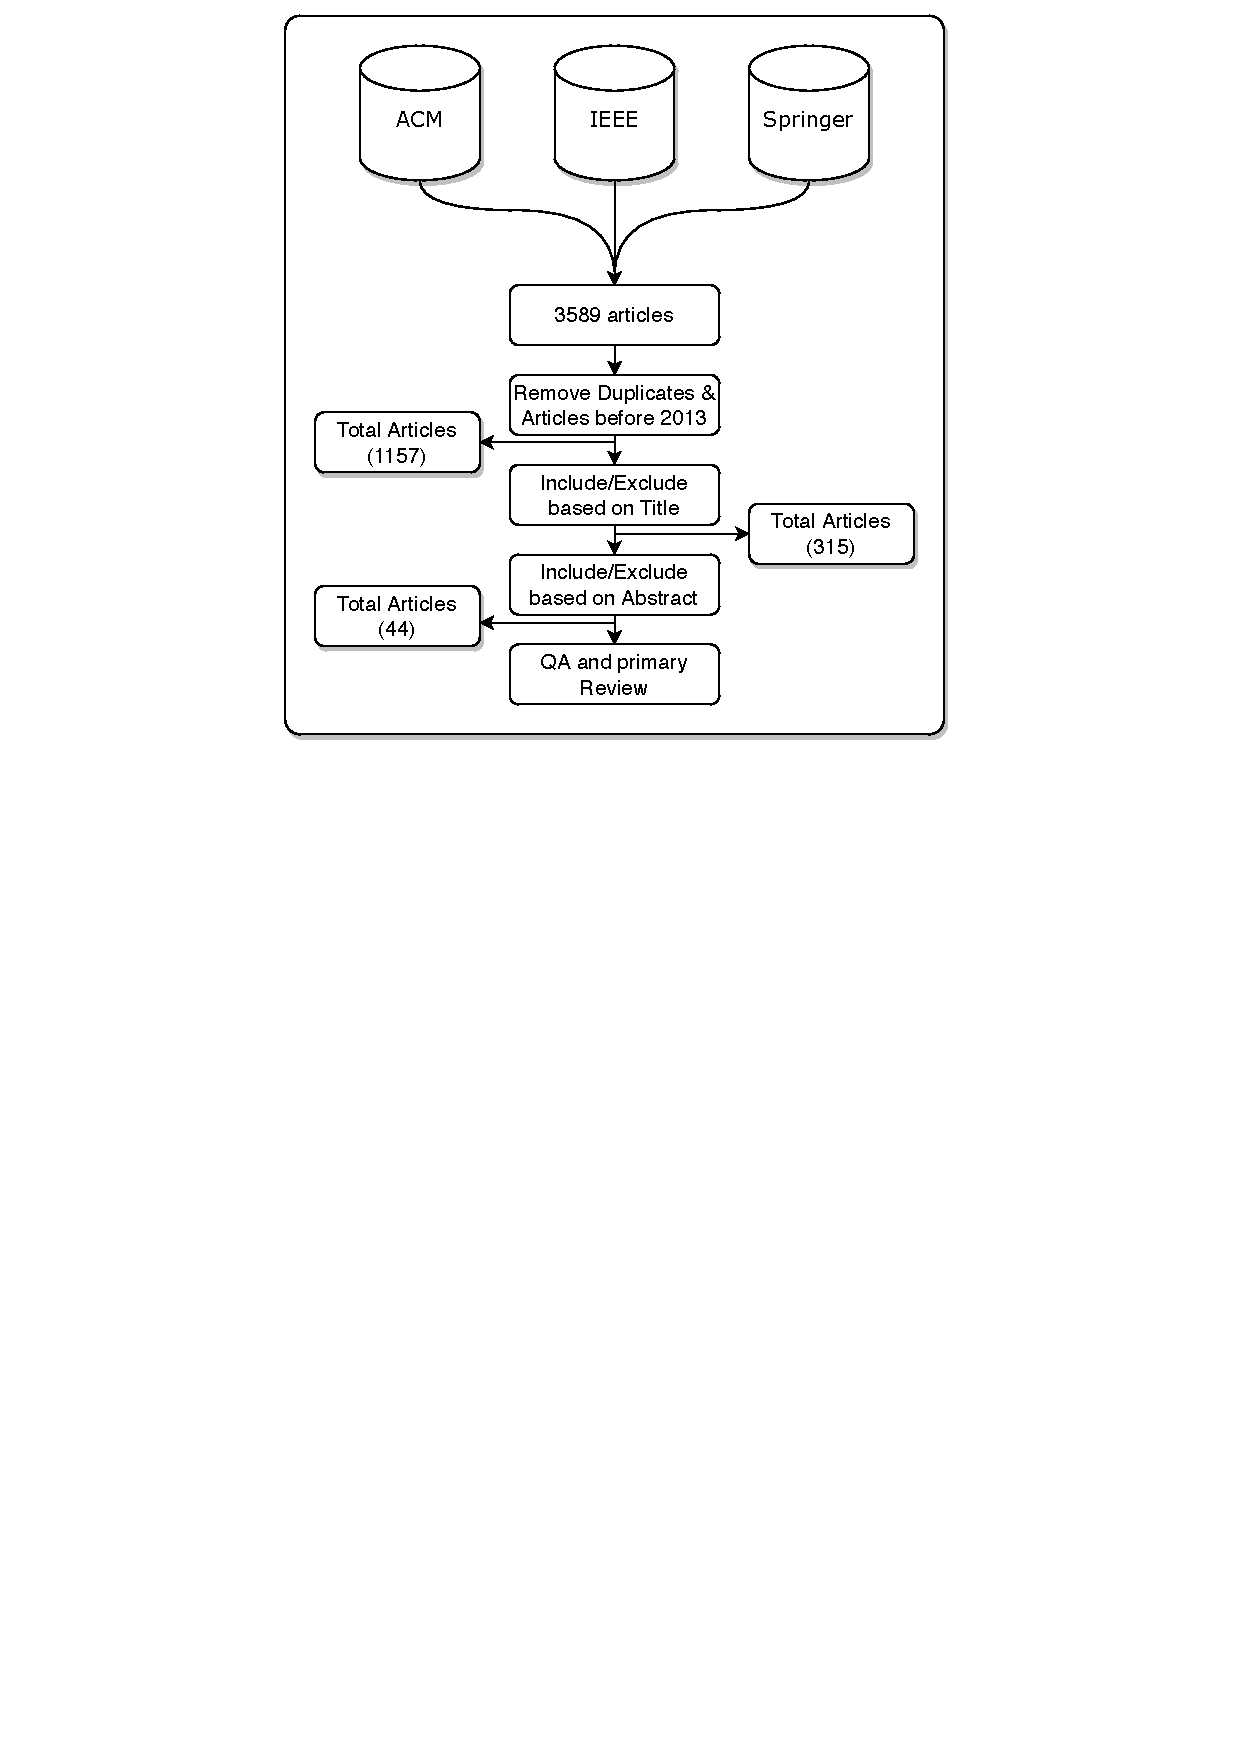
\includegraphics[trim={4.5cm 17cm 4.5cm 0},clip,width=0.465\textwidth]{images/SLRProcessVertical}
    \caption{Selection of articles - tollgate}
    \label{fig:SLRProcess}
\end{figure}

\begin{figure}[h!]
    \centering
    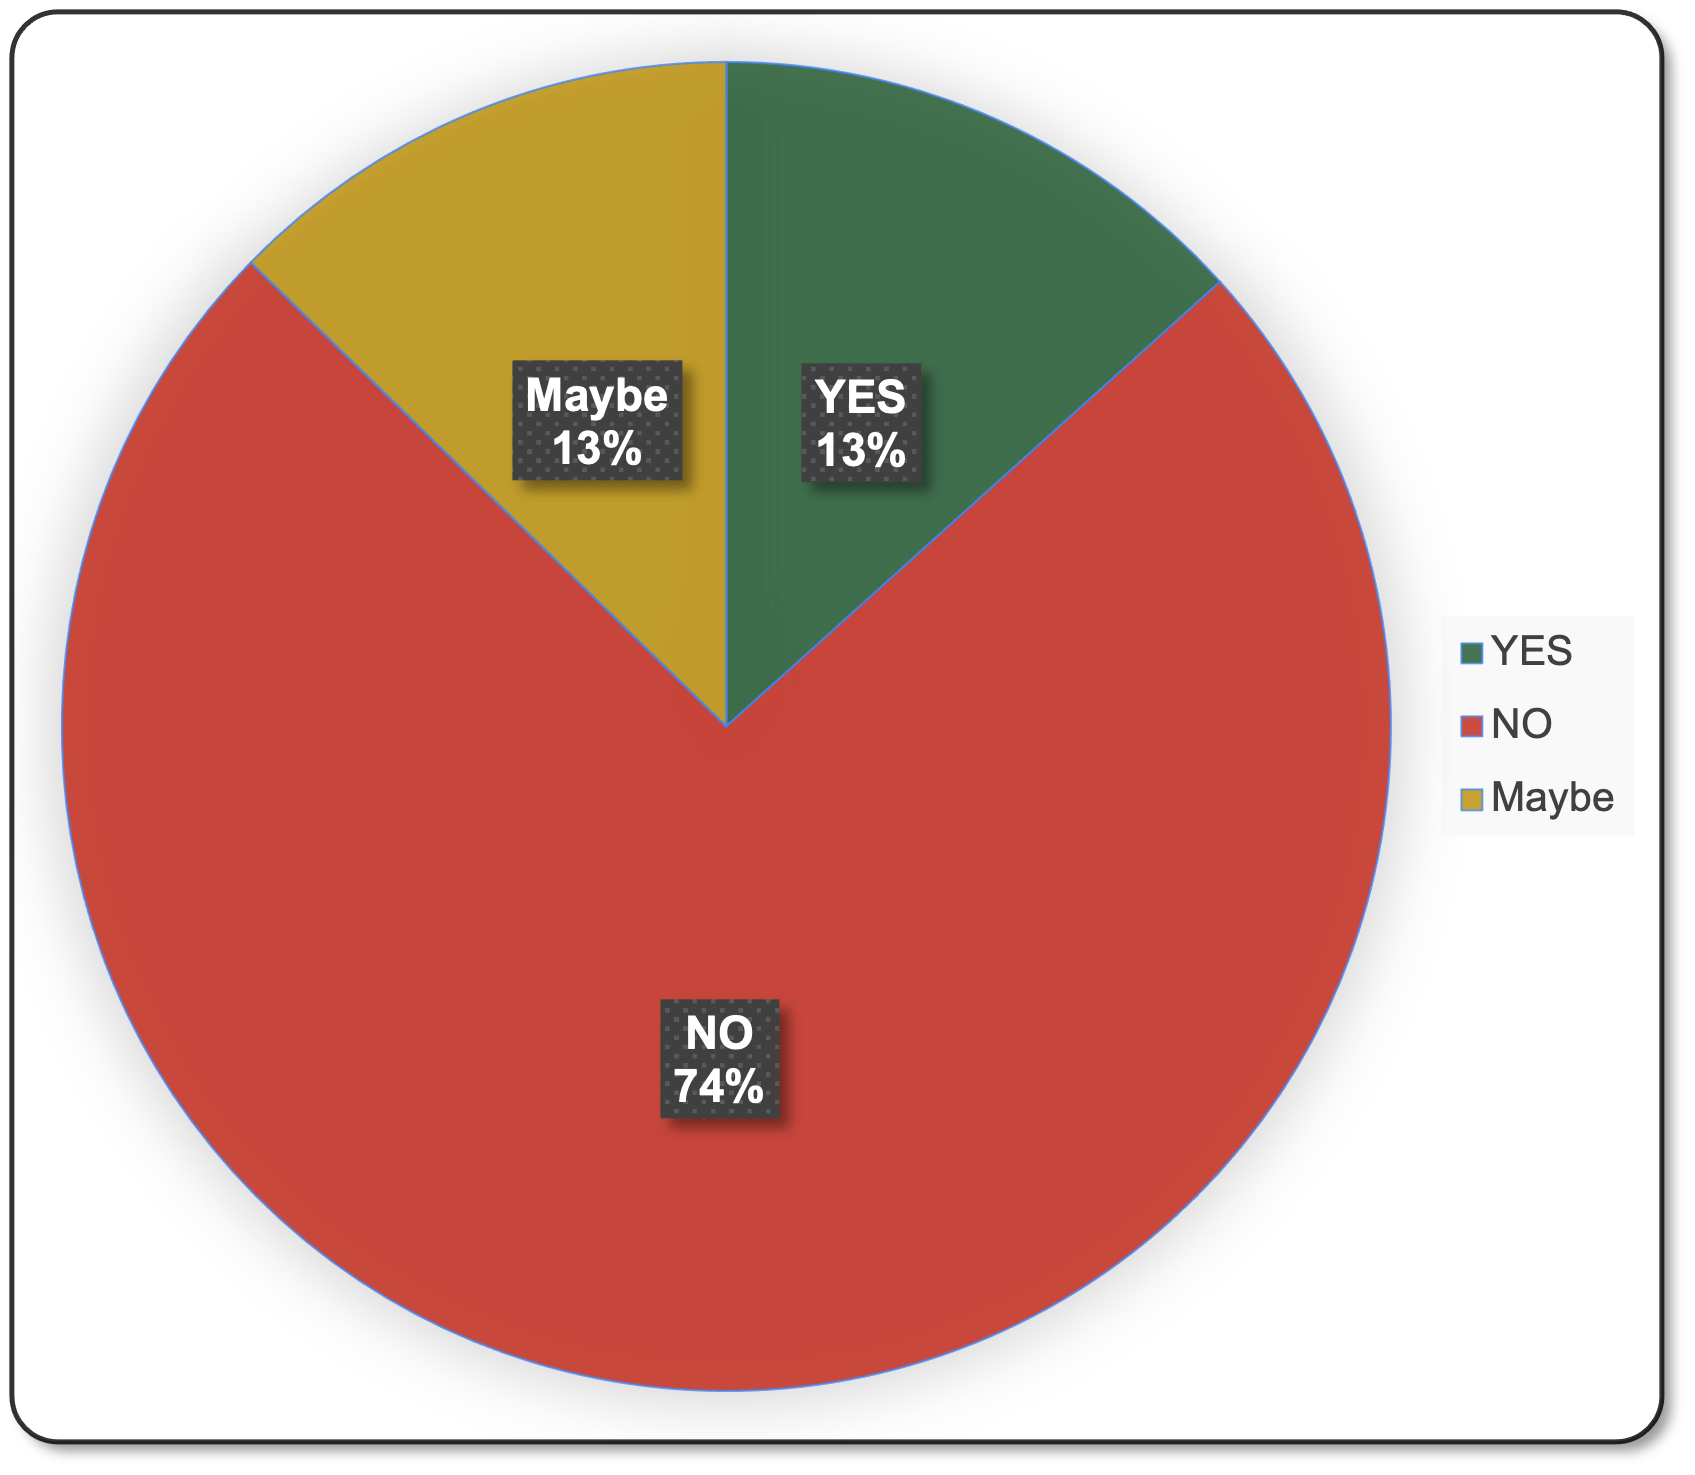
\includegraphics[width=0.45\textwidth]{images/splitQA.png}
    \caption{Split after quality assessment performed}
    \label{fig:splitQAUpdated}
\end{figure}


\paragraph{Data Extracted}
Once the most useful papers were selected, each author was tasked with extracting up to ten key points in the paper relating to process model transition.  % TODO: What else did we extract?

%\paragraph{Data Synthesis}
% "How were the data synthesised? How were differences between studies investigated? How were the data combined? Was it reasonable to combine the studies? Do the conclusions flow from the evidence?"

%\section{Reporting Phase}
% I'm fairly certain the reporting phase is just the results.




\subsection{Empirical data collection}
Two questionnaires were developed based on the key factors of process model transition identified through SLR. The first questionnaire targeted industry professionals who have undergone a software process model transition. The second questionnaire was more general and asked respondents for their thoughts and opinions on software process models that they have experience using. Both questionnaires were created in Google Forms. Participants were asked to fill out the first questionnaire if they \textbf{had} undergone a process model transition.  As a fall back, participants were asked to fill out the second questionnaire if they \textbf{had not} participated in a process model transition.

The Process Model Transition questionnaire asked each respondent sixteen questions. Questions one through three gathered context about the participant, including their role in the transition and what process model they transitioned from and to. Questions four through seven were related to trends found in RQ1. Questions eight through ten were related to trends found in RQ2. Questions eleven through fifteen were related to trends found in RQ3. The final question was an open-ended question that allowed the participant to share any relevant thoughts or opinions.

The Process Model questionnaire was used to gain more insight on whether or not a transition was successful and if the current process model had degraded in quality after a duration of time. The questions were similar to the Process Model Transition questionnaire, but were changed slightly to fit the context of the survey. The last three questions of the survey were open-ended and asked if the participant would prefer other process models versus their current one, if they had any challenges, shortcomings, or complaints about their current process model, and if they had any additional thoughts they would like to share.

\subsubsection{Data sources}

To gather real-world experience in model transitioning, the two questionnaires were sent to process model practitioners for completion. The two surveys were opened for response on April 12, 2023 and closed on April 18, 2023. There was a wide variety of the roles the respondents took, ranging from developer to manager to subject-matter expert.
% TODO: What else can we put here? Maybe we should update response period end date to 4/25 to include all 57 survey responses

\section{Findings}
The results and analyses of the SLR and survey are discussed in this section.

\subsection{SLR - Identified Challenges and Approaches}
A total of 44 primary research articles were identified in the team's systematic literature review. From these articles a total of 95 key points where extracted and grouped by their relevance to the research questions and to each other. Through grouping, 7 specific factors in process model transitions were identified and targeted in the questionnaire\cite{7477924, 9140091, 7765512, 7170402, 6702805, 8469577, 8802694, 6633979, 7302487, 8113260, 6984105, 10017407, 10049356, 7496585, 8102324, 9522254, 8498180, 8741796, 7284602, 9753613, 6986021, 9117324, 9137917, 8560640, 10.1145/1987875.1987901, 10.1145/3466933.3466962, 170231, 4293607, 8977654, 8672701, 9524860, 9049291, 9141094, 7602985, 9882761, 9337750}. The challenges are described below in more detail.
\begin{table}[htp]
    \centering
    \caption{Identified challenges in SLR}
    \label{tab:ChalAndApproach}
    \begin{tabular}{ p{1.5cm} l c c}
        \hline
        \textbf{ID}  &   \textbf{Description}    & \textbf{Paper(s)}  \\ \hline
         C1   &  Amount of training &  35 \\ 
         C2   &  Presence of a Designation Champion/Coach & 31  \\ 
         C3   &  Specific Process Model Tools & 27  \\ 
         C4   &  Process Model Modification & 24  \\ 
         C5   &  Support of Leadership/Management & 21  \\ 
         C6   &  Embracing Change & 17  \\ 
         C7   &  Dark Champions/Hindrances by Personnel & 10  \\ \hline 
    \end{tabular} \vspace{1mm}
\end{table}

The amount of training to adopt to the new process model is identified as C1. This challenge builds upon the team's abilities to adapt to a new process model and whether or not training is required. Studies highlighted the need for training for team member to understand and effectively implement the new process model and without proper training, practitioners may struggle to understand and adopt the new process model, which in the end could lead to delays and a diminished production of deliverables. 

The absence of a designated Champion/coach to guide and support the team through the transition was identified as another challenge. This person should be experienced in the process model and have the skills to ensure a successful implementation of the new process model. The champion's/coach's role would be to provide guidance and help overcome resistance to change. The champion/coach should provide ongoing support throughout the transition and to ensure the new process model is adopted successfully. 

C3 highlights the use of specific process model tools. Proper tools might not be acquired for the new process model or may be unfamiliar to the personnel. Process model tools may be used to align the project's requirements, intermediate goals and the final goal. The tools used in the new process model should be compatible with organization's existing tools and systems to minimize the impact of the transition.

Process models may need to be modified to fit an organization's unique needs, this is identified as challenge number four (C4) in the literature review. This challenge requires a thorough understanding of the existing process model and the new one to ensure smooth transition. 

Identified challenge 5 (C5) addresses lack of support from leadership/management. This challenge is identified as crucial to a smooth and successful transition. If the leadership/management of an organization does not support the team in their transition, it may result in delayed implementation of the new process model or even conclude in total failure. 

Embracing the change is another identified challenge in the SLR (C6). If practitioners are resistant to change it leads to either delays or an improper transition to the new process model. Communication is critical to this challenge and information should be shared with all involved parties including the reasons to change and what benefits this change will bring.  

The last identified challenge (C7) is dark champions/hindrance by personnel. Dark champions are individuals which are working against the transition to a new process model. Dark champion refers to a person which appear to support to transition but secretly works against the transition. Hindrance by personnel is more individuals actively resisting to transition in this case. 

\subsection{Results of Empirical Study}

\begin{figure}[H]
    \centering
    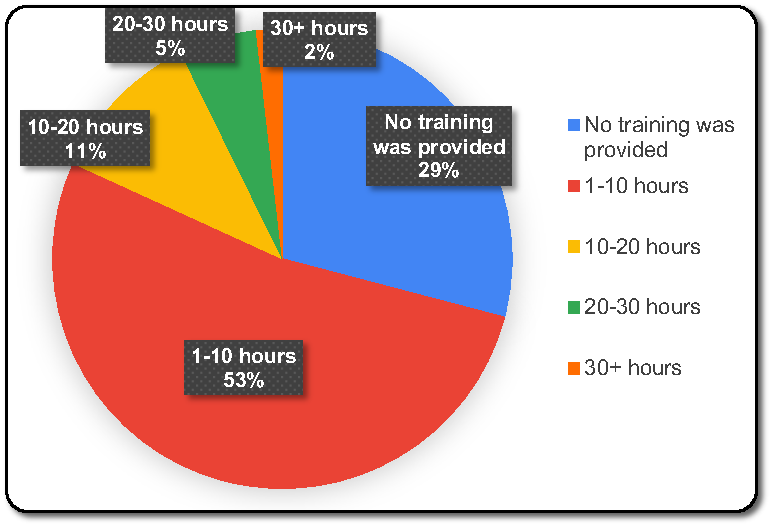
\includegraphics[width=0.45\textwidth]{images/EmpC1-Training}
    \caption{Amount of training provided}
    \label{fig:EmpC1-Training}
\end{figure}
\subsubsection{Training on the New Process Model and Its Differences}
Training is key before a transition. It allows personnel to understand their new roles or the new practices that they must adhere to without consistently being confused and creating mistakes\cite{10.1145/1987875.1987901}. According to the Fig. \ref{fig:splitQAUpdated} results, 52.73\% of participants received training on the new process model and how it differs from the old model lasting between one and ten hours. However, 29.09\%, a significant percentage, claimed to have had no instruction at all. These results emphasize the necessity for enterprises to offer proper training and support for their teams in order to allow a smoother and more efficient transition. They also show the various levels of training provided to employees during the transition to a new process model.
\begin{figure}[H]
    \centering
    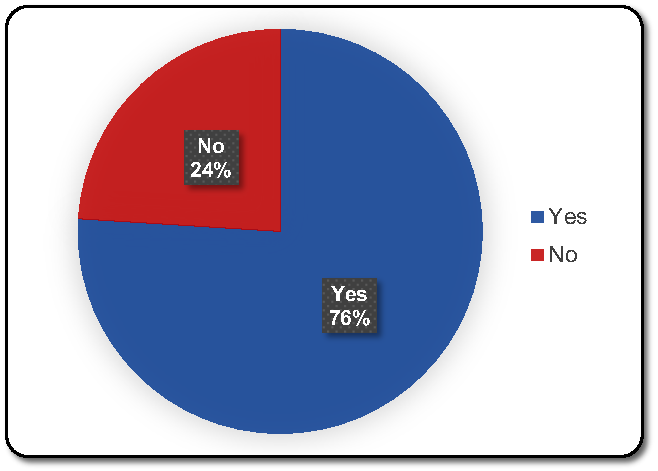
\includegraphics[width=0.45\textwidth]{images/EmpC2-Coach}
    \caption{Was there a designated "Champion/Coach" of the transition? }
    \label{fig:EmpC2-Coach}
\end{figure}
\subsubsection{Presence of a Designated Champion/Coach During the Transition}
The Data from Fig. \ref{fig:EmpC2-Coach}, 76\% of respondents to the study said that there was a "Champion/Coach" assigned to the transition who was responsible for answering questions and facilitating the process. However, 24\% of the respondents said that there wasn't a dedicated person in place. These results emphasize the value of having a committed person lead and assist teams as they switch to a new process paradigm. The presence of a Champion/Coach can greatly aid in addressing issues, promoting understanding, and ensuring an organization's transformation is easier and more successful\cite{8672701, 9137917}.
\begin{figure}[H]
    \centering
    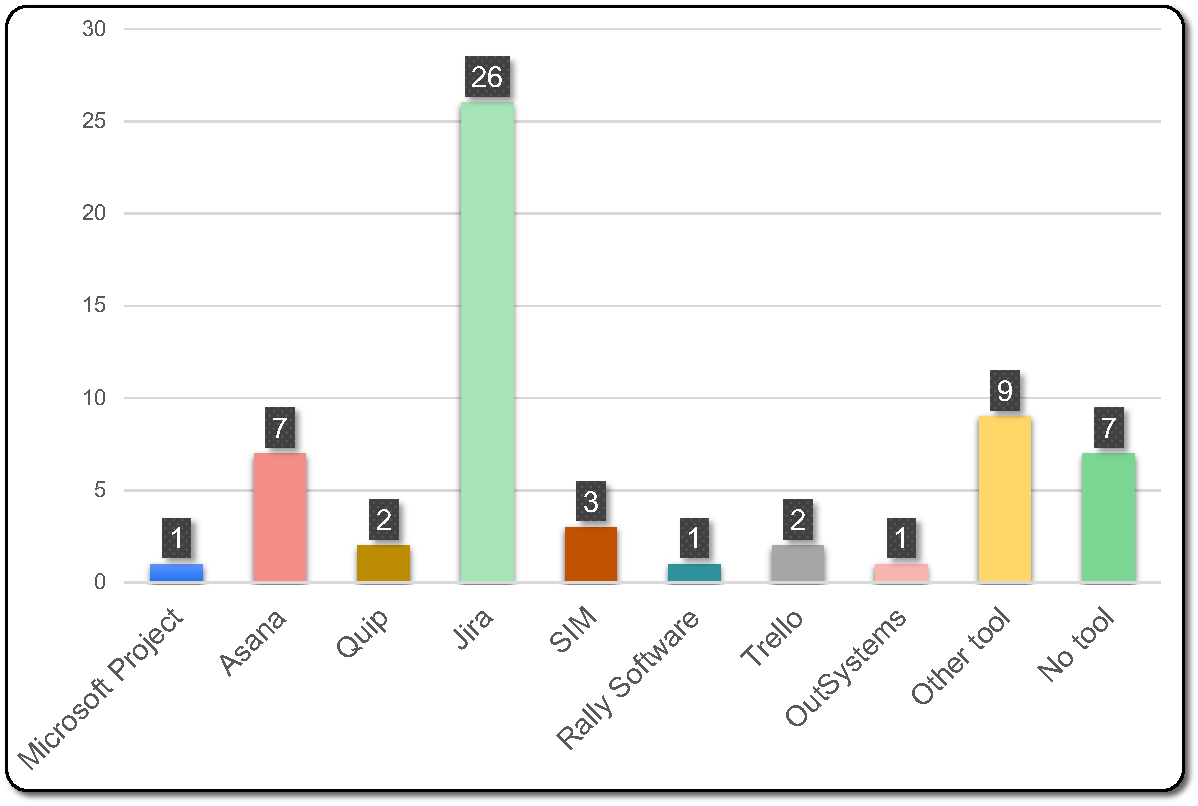
\includegraphics[width=0.45\textwidth]{images/EmpC3-Tools}
    \caption{Tools that benefited transition}
    \label{fig:EmpC3-Tools}
\end{figure}
\subsubsection{Tools Utilized for Facilitating the Transition Process}
Proper tracking tools and organization tools are important during and after a transition\cite{9522254}. Numerous tools were employed to aid the changeover process, as shown by the survey findings in Fig. \ref{fig:EmpC3-Tools}. Jira was used by respondents the most frequently (26), followed by Asana (7). Microsoft Project (1), Quip (2), SIM (3), Rally Software (1), Trello (2), and OutSystems (1) are a few additional tools that have been cited. In addition, 9 respondents mentioned utilizing additional tools, while 7 respondents said they didn't use any particular tools at all during the move. The findings show that there are a diverse range of tools available in aiding the transitions.
\begin{figure}[H]
    \centering
    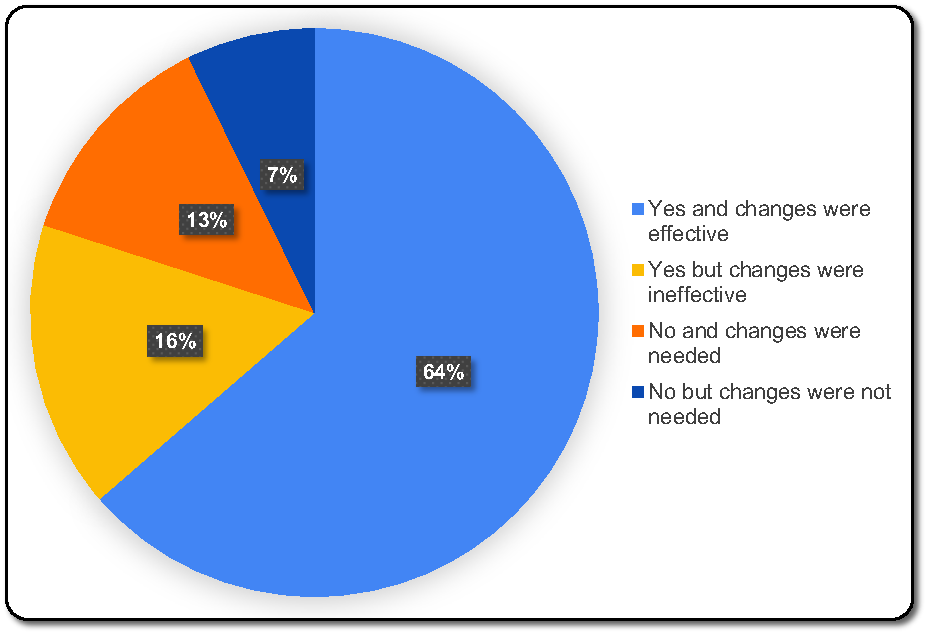
\includegraphics[width=0.45\textwidth]{images/EmpC4-Modifications}
    \caption{Were there any modifications to the new process model to better fit the specific needs of the organization?}
    \label{fig:EmpC4-Modification}
\end{figure}
\subsubsection{Modification to the new process model}
According to Fig. \ref{fig:EmpC4-Modification} of the data, most businesses modified the new process model in some way, and the majority of these alterations were thought to be successful. However, a sizable portion of respondents continued to express the opinion that the improvements were either unnecessary or ineffective. This response was lower than anticipated given the emphasis of certain agile process models being welcoming to process model modification\cite{6615211}. Here the results of low hours of training or lack of quality training are seen due to ineffective employment of agile principles.
\begin{figure}[H]
    \centering
    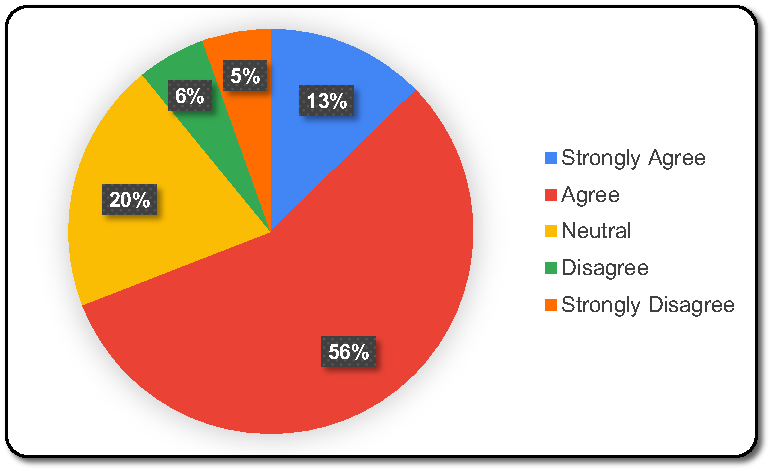
\includegraphics[width=0.45\textwidth]{images/EmpC5-LeaderConfidence}
    \caption{Leadership had confidence in the team(s) and was fully supportive in the transition}
    \label{fig:EmpC5-LeaderConfidence}
\end{figure}
\subsubsection{Leadership Support and Confidence During Transition}
A recurring theme found throughout the papers identified through the team SLR, support of management and leadership during a process model transition has great impact upon it success\cite{7765512}. According to the survey results shown in Fig. \ref{fig:EmpC5-LeaderConfidence}, 69\% of participants either agreed or strongly agreed that the leadership had faith in the team(s) and provided unwavering support during the transition. However, 11\% of respondents disagreed or strongly disagreed, while 20\% had no opinion. This shows that, for the most part, leadership helped with the change, but there is still a sizable group of businesses where that support may not have been as strong or meaningful.
\begin{figure}[H]
    \centering
    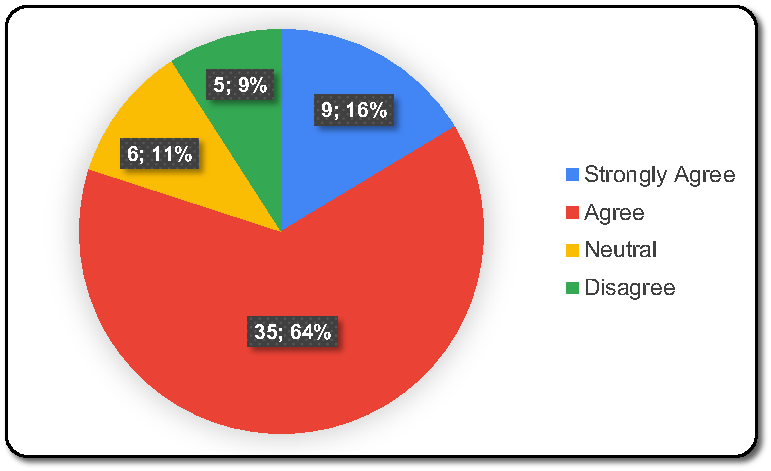
\includegraphics[width=0.45\textwidth]{images/EmpC6-EmbracingChange}
    \caption{The new process model and changes were embraced by my team}
    \label{fig:EmpC6-EmbracingChange}
\end{figure}
\subsubsection{Team Embracement of New Process Model and Changes}
Without motivated personnel, the process model transition can be a grueling process and likely to result in failure. Thus it is exceptionally important for organization to motivate their personnel to embrace change rather than fight it\cite{7496585}.The data in Fig. \ref{fig:EmpC6-EmbracingChange} shows 80\% of the respondents either agreed or strongly agreed that their team as a whole embraced the new process paradigm and adjustments. 9\% of respondents disagreed with the statement, while 11\% stayed indifferent. Nobody who responded disagreed strongly. These results indicate that teams were generally responsive to the new process model and adjustments, emphasizing the significance of group adaptation and collaboration during a transition.
\begin{figure}[H]
    \centering
    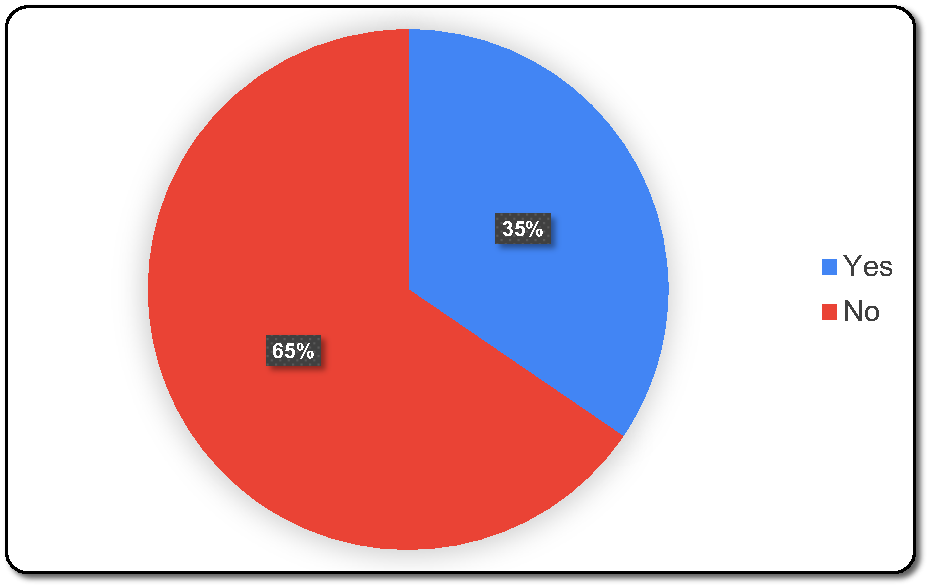
\includegraphics[width=0.45\textwidth]{images/EmpC7-Hindrances}
    \caption{There were personnel that did not like the transition and hindered its progress or success}
    \label{fig:EmpC7-Hindrance}
\end{figure}
\subsubsection{Impact of Personnel Resistance on Transition Progress and Success}
According to the survey results displayed in Fig \ref{fig:EmpC7-Hindrance}, 35\% of respondents said that certain employees disliked the transition and hampered its performance. In contrast, 65\% of respondents said they were unaffected by this problem. These results highlight the possible influence of personal resistance on the success and advancement of a change to a new process model. To promote a smoother and more successful transition, it is critical for employers to proactively manage employee resistance through effective communication, training, and support.

\subsubsection{Connections among Responses}
The following section compares relevant responses next to each other in order to illustrate the correlation between them.

\begin{figure}[H]
    \centering
    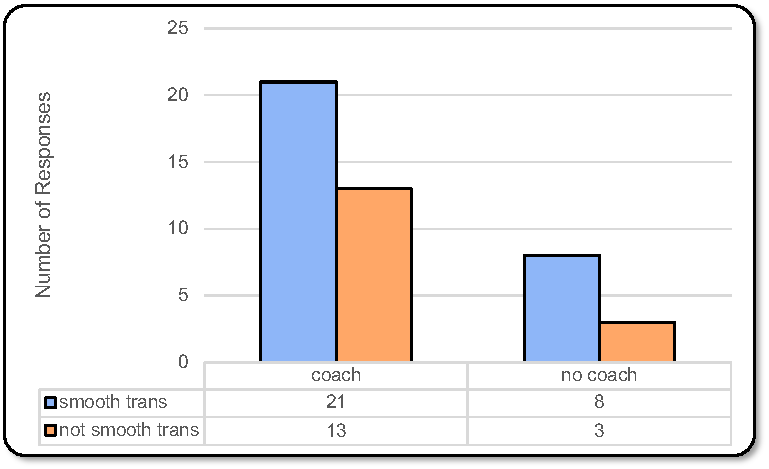
\includegraphics[width=0.45\textwidth]{images/Emp-CoachVsSmoothTrans}
    \caption{Presence of a coach and smoothness of transition}
    \label{fig:CoachVsSmooth}
\end{figure}

As illustrated in Fig. \ref{fig:CoachVsSmooth} did the majority of respondents in the empirical study indicate the transition and implementation of a new software process model to be smooth. It's interesting to compare this to the use of a designated coach assigned to facilitate the new process, answer questions and provide guidance. The data shows that the use of a designated coach does not necessarily make the transition smoother compared to not having a coach. The proportion between smooth transition and not smooth transition remain the same with or without a designated coach. An additional round of questionnaires my be needed to drill down further on these findings. More information is needed to determine if these coaches were truly acting as coaches or if they were just a person who knew the most about a given process model ans subsequently tasked with assisting in the transition.

\begin{figure}[H]
    \centering
    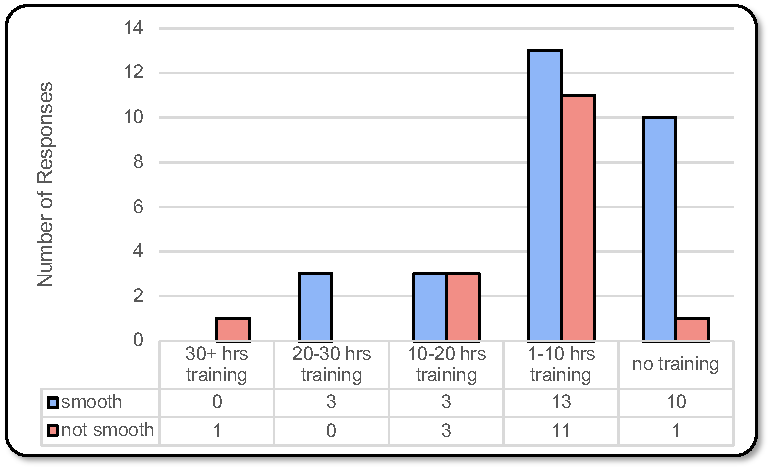
\includegraphics[width=0.45\textwidth]{images/Emp-TrainingVsSmoothTrans}
    \caption{Relationship between training duration and smoothness of transition}
    \label{fig:TrainingVsSmooth}
\end{figure}

According to data displayed in Fig. \ref{fig:TrainingVsSmooth} which illustrates the relation between the smoothness of the transition in relation to the amount of training provided or received in the implementation of a new process model, a more extensive amount of training does not necessarily equal a smoother transition. The majority of the respondents did either get no training or 1-10 hours of training. On the other end where 30+ hours of training were provided the respondents did not experience a smooth transition. The respondents receiving 0 to 10 hours of training were more likely to experience a smooth transition. This data could indicate that most of the respondents already were slightly familiar with the new process model being implemented or a lack of management support. 

As illustrated on Fig. \ref{fig:SupportTransHeat} there is a correlation between how supportive the leadership at the company is and how smooth the transition was. This indicates the importance of trust and confidence in the team from the leadership's side which encourage the team to transition and in the end will make the transition worth it. This also goes the other way where the team should embrace the transition which would make it more worth it according to Fig. \ref{fig:EmbraceTransHeat} illustrating the correlation between worth of the transition and whether or not the team embraced the transition.

\begin{figure}[H]
    \centering
    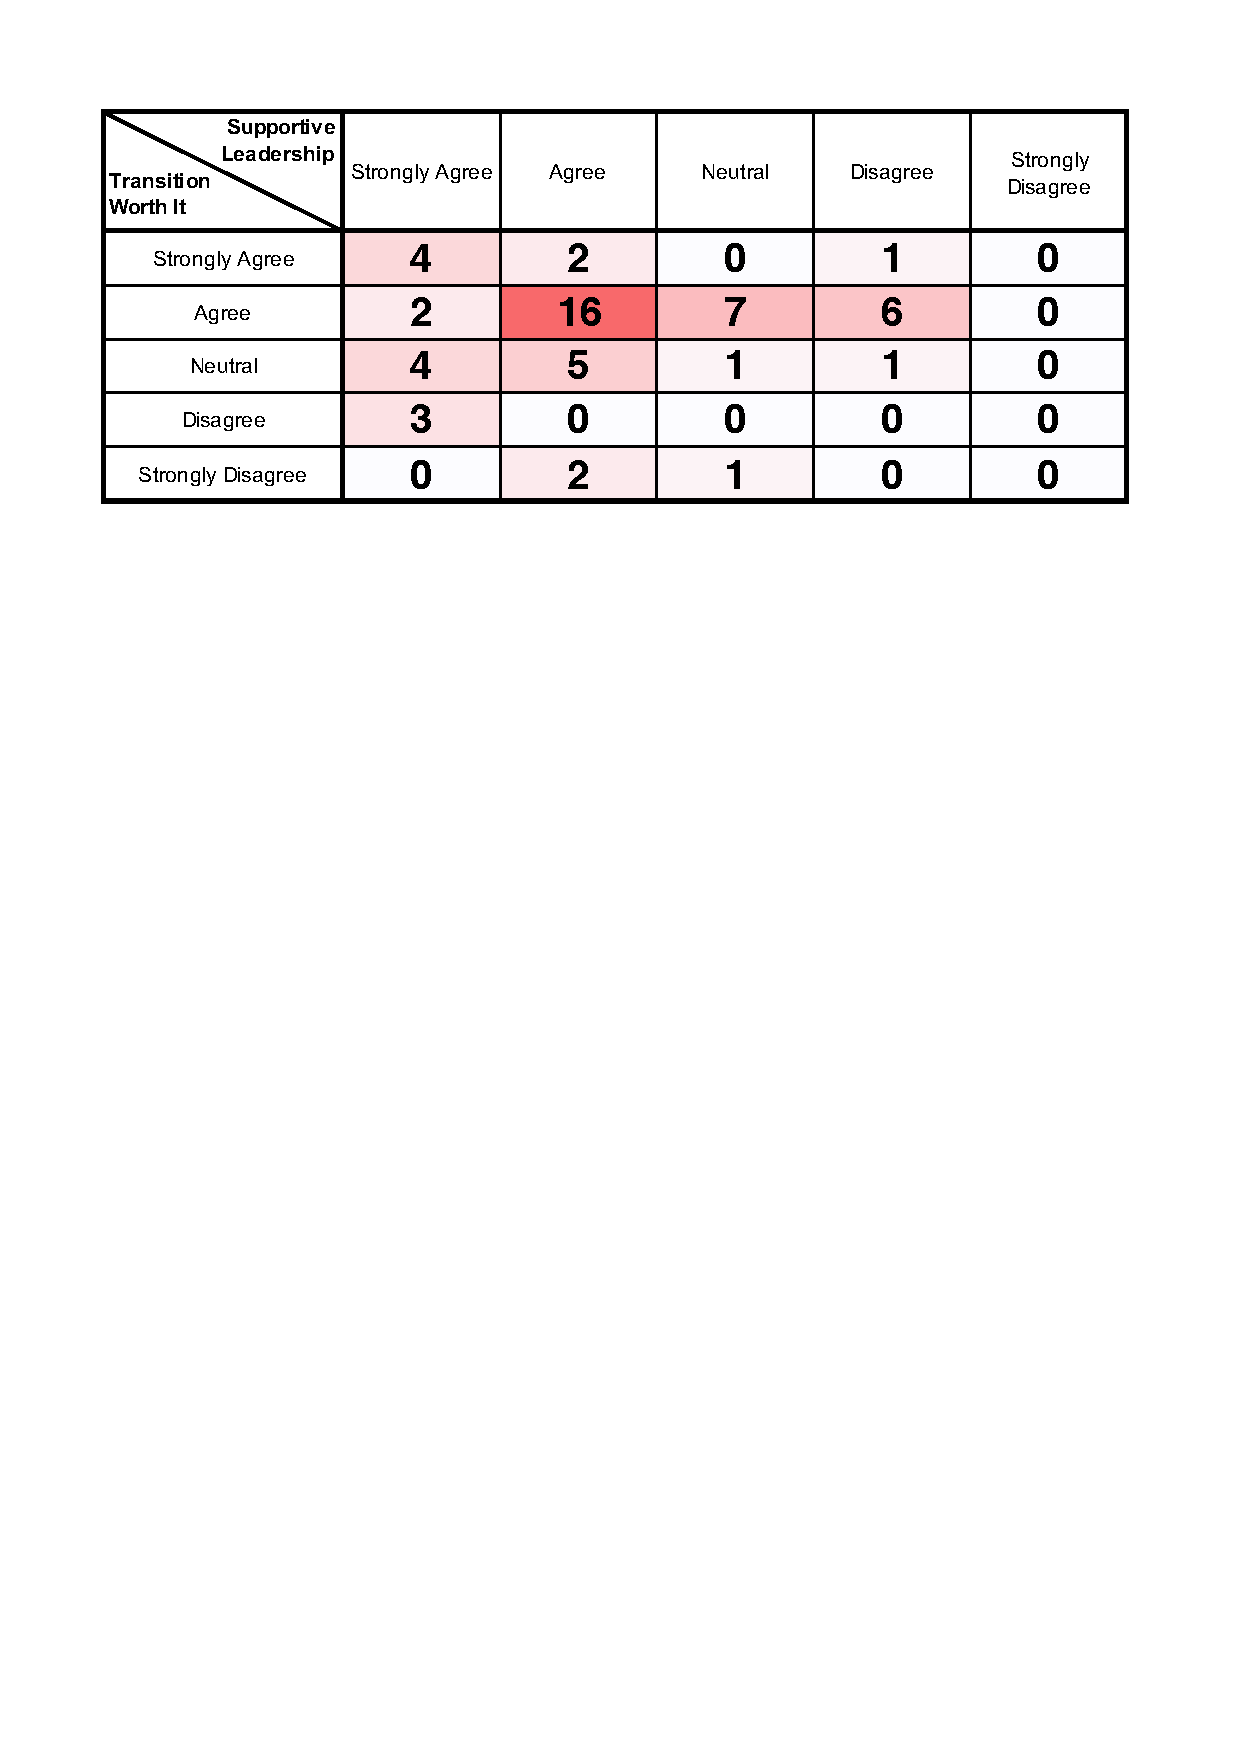
\includegraphics[trim={1.5cm 21cm 1.5cm 0},clip,width=0.45\textwidth]{images/Emp-SupportTransHeat}
    \caption{Correlation between leadership support under transition and whether the transition was worth it or not}
    \label{fig:SupportTransHeat}
\end{figure}


\begin{figure}[H]
    \centering
    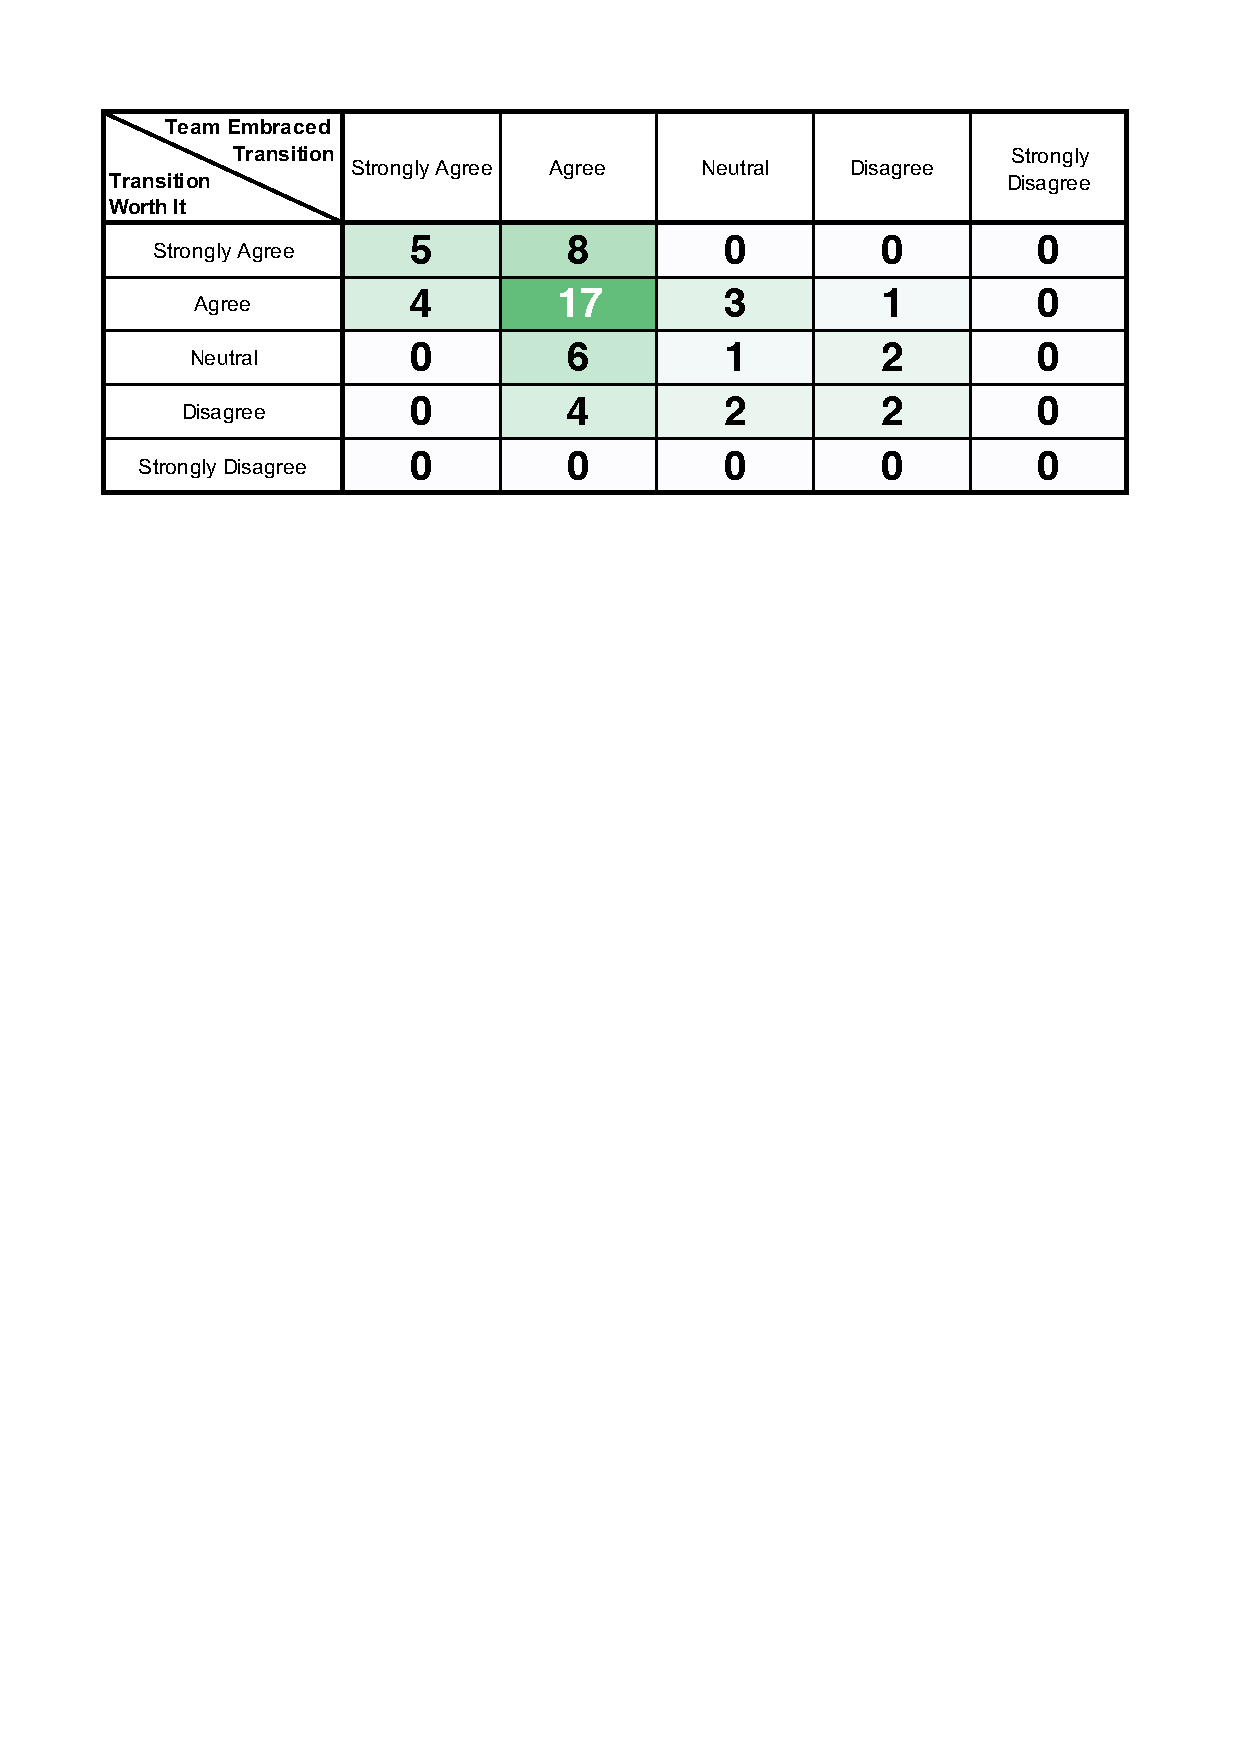
\includegraphics[trim={1.5cm 21cm 1.5cm 0},clip,width=0.45\textwidth]{images/Emp-EmbraceTransHeat}
    \caption{Correlation between team embracing transition and whether transition was worth it or not}
    \label{fig:EmbraceTransHeat} 
\end{figure}


\section{Discussion}

Through our SLR and subsequent survey we identified the following answers to our original research questions.

\textbf{RQ1:} The existing approaches to process model transitioning in software engineering were identified, including the use of documentation and guidelines, training and education programs, process tailoring and customization, and the use of process modeling tools. But it was found that the current body of research focuses almost entirely on transitions from waterfall to agile, and does not include other transitions such as kanban to scrum or the introduction of a formal process model for the first time. 

\textbf{RQ2:} The challenges of process model transitioning in software engineering were also observed, such as resistance to change from employees, lack of awareness and understanding of new process models, difficulties in aligning existing practices with new models, and the need for additional resources and efforts for transitioning. These challenges shed light on the barriers and obstacles that organizations face when transitioning to a new process model, providing a better understanding of the difficulties and complexities involved in the transition process.

\textbf{RQ3:} The benefits of process model transitioning in software engineering were also identified in the observations, including improved productivity, better quality of software products, increased efficiency, and enhanced collaboration among team members. These benefits highlight the motivations and advantages of organizations in choosing to transition to new process models, providing insights into the positive outcomes that can be achieved through process model transitioning.

Furthermore, in answering our primary research questions, our research generated several key insights.

1) Counter-intuitively, the amount of training that team members received on the new process model and its differences did not directly correlate to better outcomes.  This suggests an area of further research.
2) Having a designated "Champion/Coach" during the transition process is beneficial, as it helps answer questions and facilitate the transition. 76\% of respondents in the study reported having a Champion/Coach, while 24\% did not. This emphasizes the value of having a dedicated person to lead and assist teams during the transition.
3) Utilizing tools for tracking and organization can aid the transition process. The survey found that various tools were used, with Jira being the most commonly used tool, followed by Asana. This shows the availability of a diverse range of tools to aid in transitions.
4) Most businesses made modifications to the new process model to better fit their specific needs, and the majority of these modifications were considered successful. However, a significant portion of respondents expressed that the modifications were unnecessary or ineffective, which was lower than anticipated based on the agile process models' emphasis on welcoming modifications.
5) Leadership support and confidence during the transition process is important for success. 69\% of respondents agreed or strongly agreed that leadership had faith in the team(s) and provided unwavering support during the transition, while 11\% disagreed or strongly disagreed. This shows that while leadership support was generally present, there were still some businesses where it may not have been as strong.
7) Team embracement of the new process model and changes is crucial for success. 80\% of respondents agreed or strongly agreed that their team embraced the new process paradigm and adjustments, while 9\% disagreed. This highlights the importance of motivating personnel to embrace change rather than resist it during the transition process.

\section{Future Work}
The ultimate goal of this research team is to create a comprehensive checklist for selecting a process model and a guide for successfully transitioning from one process model to another. To achieve this goal, our future research will focus on conducting a larger systematic literature review to identify the most commonly used process models and their associated strengths and weaknesses. Additionally, we will conduct a larger empirical study spanning more personnel from various global locations and organizational sizes to evaluate the effectiveness of different transition techniques and identify the common challenges and barriers organizations face during the process model transition.

The development of a comprehensive checklist and guide for selecting and transitioning between process models could provide numerous benefits to businesses. Firstly, having a clear understanding of the strengths and weaknesses of different process models can help organizations select the most appropriate process model for their specific needs, improving the efficiency and effectiveness of their business processes. Secondly, a well-designed transition guide can help organizations minimize the disruption and negative impact of transitioning to a new process model, ensuring a smooth and successful transition.

Moreover, a standardized checklist and guide can help organizations save time and resources by providing a clear and concise road map for selecting and transitioning between process models, reducing the need for extensive trial-and-error testing and troubleshooting. Finally, a standardized approach to process model selection and transition can improve communication and collaboration within an organization, as employees across different departments and teams can rely on a shared understanding of the process model selection and transition process. Overall, the development of a comprehensive checklist and guide for selecting and transitioning between process models can help organizations improve their business processes, enhance their competitiveness, and drive success in the long term.

\section{Conclusion}
In conclusion, our research team's systematic literature review and empirical study provided consistent and complementary insights into the process of selecting and transitioning between process models. Our systematic literature review identified the most commonly used process models and the challenges when transitioning to them, while our empirical study evaluated the effectiveness of different transition techniques and identified common challenges and barriers faced by organizations during the process model transition.

Our study findings suggest that a standardized approach to process model selection and transition, aided by a comprehensive checklist and guide, can provide significant benefits to businesses. The findings from our literature review and empirical study were consistent with each other, which adds to the strength of our overall research. By selecting the most appropriate process model and transitioning smoothly to new models as needed, organizations can improve their business processes, enhance their competitiveness, and drive success in the long term. Moving forward, we hope that our research will contribute to the development of practical and accessible tools for organizations to improve their process model selection and transition processes, ultimately leading to improved business performance and success.

\printbibliography
\end{document}
